\chapter{Overview of Catastrophic Indicators}

\section{General Terminologies used for Stability Assessment}
\begin{itemize}
\item \textbf{Swing Equation-}
This is the equation that describes the relative motion of the rotor (Load Angle $\delta$) with regard to the stator field as a function of the time \cite{7}.
\begin{equation}
f(\delta,\omega)=\begin{cases}
\frac{d\delta_i (t)}{d(t)} = \omega_i (t) - \omega \\
\frac{d\omega_i (t)}{d(t)} = \frac{1}{M_i}[P_{m_i} (t) - P_{e_i} (t)]
\end{cases}
\end{equation}
%Where, \(\omega_i, \delta_i, P_{m_i}, P_{e_i}\) and \(M_i\) is the speed, Rotor Angle, Electrical Power and Mechanical Power of the ith generator.
Where, \hspace{0.7 cm}\(\omega_i\) - Speed of \(i_{t_h}\) generator\\
\tab\tab \(\delta_i\) - Rotor Angle of \(i_{t_h}\) generator
\\\tab\tab \(P_{e_i}\) - Electrical Power of \(i_{t_h}\) generator
\\\tab\tab \(P_{m_i}\) - Mechanical Power of \(i_{t_h}\) generator
\\\tab\tab \(M_i\) - Cumulative Inertia of \(i_{t_h}\) generator
\\\tab\tab \(\omega\) - Synchronous Speed or Speed of the System

\item \textbf{Center of inertia of an Area-}
For \(N_g\) generators in an \(i_{th}\) area, the comparing Center of Inertia can be characterized as \cite{8}:-
\begin{equation}
\delta_{COI_i} = \frac{1}{M_i} \sum_{k=1}^{N_{g_i}} M_k \delta_k
\end{equation}\begin{equation}
M_i = \sum_{k=1}^{N_{g_i}} M_k 
\end{equation}
%Where, \(M_k , \delta_k, M_k\) – Inertia, Rotor Angle, Cumulative Inertia of \(k_{t_h}\) Generator.\\
%\(N_{g_i}, M_k\) – Number of Generators, Cumulative Inertia of ith area
Where,\hspace{0.75 cm} \(\delta_k\) - Rotor Angle of \(k_{th}\) generator
\\\tab\tab \(N_{g_i}\) - Number of Generators in the \(i_{th}\) area
\\\tab\tab \(M_i\) - Cumulative Inertia of the \(i_{th}\) area
\\\tab\tab \(M_k\) - Inertia of \(k_{th}\) generator

\item \textbf{Center of inertia of the System-}
The comparing Center of Inertia for \(N_{area}\) coherent areas in a system can be written as \cite{8}:-
\begin{equation}
\delta_{COI_System} = \frac{1}{\sum_{i=1}^{N_{area}} M_i } \sum_{i=1}^{N_{g_i}} M_i \delta_{COI_i}
\end{equation} 
\item \textbf{Sensitive indicators for Stability Analysis-}\begin{equation}
\delta_{k}^{COI_i} = \delta_k - \delta_{COI_i} 
\end{equation}\begin{equation}
\delta_{i}^{COI_System} = \delta_i - \delta_{COI_System} 
\end{equation}Where, The relative rotor angle deviation of a generator related to its area and an area referred to its system are \(\delta_{k}^{COI_i}\) and \(\delta_{i}^{COI_System}\), respectively \cite{9}.



\end{itemize}


\section{Catastrophic Indicators}\label{Catastrophic Indicators}
\subsection{Indicator based on Coherency}
DSA contingency screening may benefit from indicators based on the concept of coherency. Considering the lack of a clear description, the idea of coherency is quite simple. Following fault-clearing, coherency is defined as the tightness of all generator rotor angles (connected to the centre of inertia COI from now on). Case A is more coherent than Case B if the angles of all generators in Case A are nearer to the COI after fault-clearing than that in Case B. As according \cite{EPM}, stable instances are significantly more intelligible than unstable cases. The performance index can be written as follows using the Coherency-based indicator:

\begin{equation}
Performance \; Index = max\big(\theta_i(t)\big)-min\big(\theta_i(t)\big) \label{IS}
\end{equation}
\tab If\tab  \textit{Performance Index } \(\ggg\) 0 : System Unstable\\
\tab Where, \hspace{0.7 cm}\(i = 1, 2, 3, ........, N_g\) \\
\tab\tab\tab \(t_{cl} \leq t \leq t_{cl}+T\) 
\\\tab\tab\tab \(t_{cl}\) - Fault clearance time. 
\\\tab\tab\tab \(N_g\) -  Total number of generators.
\\\tab\tab\tab \(T\) - Length of short period after fault clearing

\subsection{Indicator based on Transient Energy Conversion}
In generally, the transient energy presented in transient study includes kinetic and potential energy. The transient kinetic energy of a generator is determined by its speed. The transient potential energy is made up of the location power of all rotors respect to the COI, magnetic energy, and dissipation energy, the other two of which are linked to the transmission system. Once a problem has been fixed, transient stability is a measurement about whether or not the generators in the system lack synchronism. Obviously, the system's separation rises as a consequence of the temporary kinetic energy supplied by the fault. Only the changed kinetic energy, as per the results, leads to system isolation.The excess kinetic energy supplied into the system can be "taken," and the system will not lost synchronism, instead achieving a new stable equilibrium position \cite{EPM}, if the system has sufficient potential energy capability. The performance index based on Transient Energy Conversion is depicted in the eqn. below:

\begin{equation}
Performance \; Index = max\big(V_{ke}(t)\big) - min\big(V_{pe}(t)\big)
\end{equation}
\tab If\tab  \textit{Performance Index } \(\ggg\) 0 : System Unstable\\
\tab Where, \hspace{0.7 cm}\(t_{cl} \leq t \leq t_{cl}+T\) 
\\\tab\tab\tab \(V_{ke}\) - Transient Kinetic Energy.
\\\tab\tab\tab \(V_{pe}\) - Transient Potential Energy.
\\\tab\tab\tab \(t_{cl}\) - Fault clearance time. 
\\\tab\tab\tab \(N_g\) -  Total number of generators.
\\\tab\tab\tab \(T\) - Length of short period after fault clearing

\subsection{Indicator based on Dot Products (CSA)}
To ensure grid security during cascaded events and extreme scenarios, system operators must undertake dynamic security assessments. The CSA index, or \textbf{\textit{Contingency Severity Assessment}}, is one of the Exit-point approaches \cite{EPM} of dot product of system variables. The considered dot-product signal includes speed deviation and phase angle in the COI reference frame. The TEF's starting point is indicated by the index. \cite{CSA} provides a way for CSA to prioritise severe contingencies, in contrast to typical offline simulations. A portion of the procedure involves developing a set of fuzzy rules based on extracting time-domain and frequency-domain information from phasor data. On the other hand, putting together a network-specific and compact collection of fuzzy rules takes effort and is prone to errors. A systematic approach for classifying fuzzy rules is proposed \cite{CSA_WASI} to improve accuracy, reaction time, and performance for SA. The simplified equation below represents the CSA indicator.


\begin{equation}\label{CSAeqn}
C(t) = \sum_{i=1}^{N_{area}} \omega_i(t)[\delta_i(t) - \delta_i(0^+)]
\end{equation}

The spectral density can be computed using this dot product (notice its utilisation while deriving WASI index, which is described in sec. \ref{WASIsec}).

\subsection{Wide Area Severity Index (WASI)}\label{WASIsec}
It is essential to catch the shortcoming severity of an area when power move level builds due to a great extent interconnected network. It is characterized as the logarithm of  power spectral density of dot product, CSA (Contingency Severity Assessment). At high power changes, the sign energy shows an exponential increase, which can be captured using a log-linear relationship with power change.It performs better in positioning the contingency in light of a t = 1sec or t = 2sec span \cite{CSA_WASI}. Fig.  \ref{fig_WASI} shows a block diagram for computing frequency domain severity index(WASI). This feature can be expressed as:
\begin{equation}
Fast WAST(T) = log(max_{t \; \in \; [0^+,T]}(max_i(PSD(C_i(t)))))
\end{equation}

\begin{figure}%[!t]
\centering
\scalebox{1.3}{
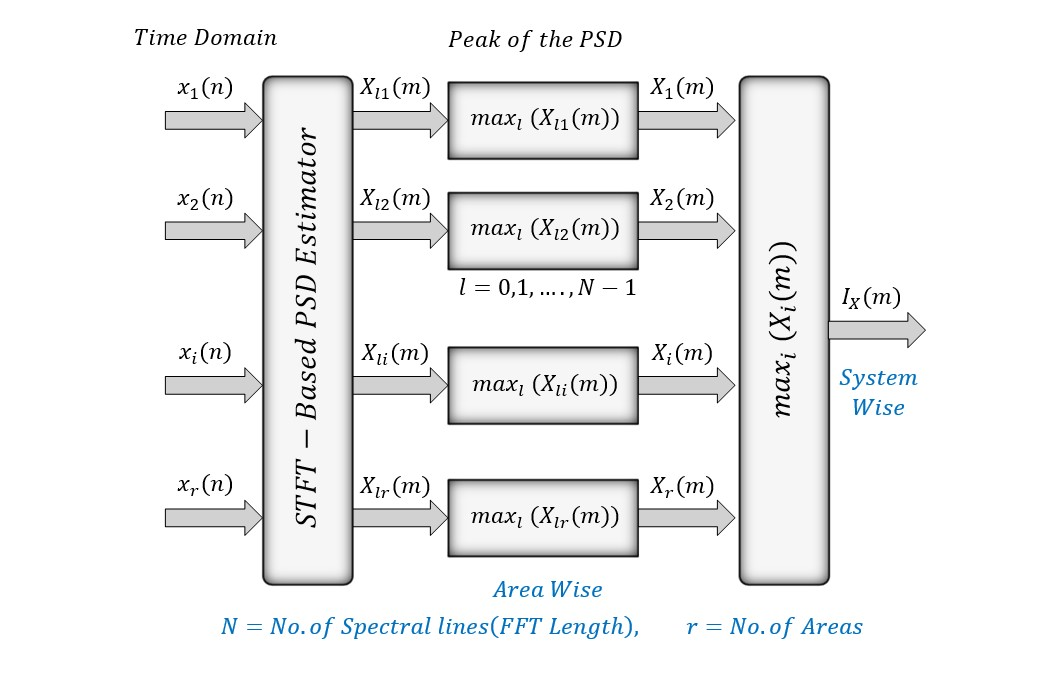
\includegraphics [width=4in] {WASI}
}
\caption{Computation of frequency-domain-based WASI}
\label{fig_WASI}
\end{figure}

\subsection{Inter-area Stability Prediction Index (ISPI)}
\label{ISPI_Intro}
In a network that is interconnected, it is critical to analyse interarea stability in light of grid contingencies. An ISPI is defined \cite{ISPI} in the time domain using two engineering metrics, namely voltage-magnitude change (reduction) and phase-angle movement (separation). This index can be used in place of the previously stated WASI, which is defined in the frequency domain.
\subsubsection{Thresholds values}
By conducting an electrical assessment in the system under consideration, it is able to ascertain angular deviations from ECOI that are vital for the system $\delta cri$, i.e. angular deviations from ECOI which can carry the system nearer to blackout when it is attained, and the maximum angular variations from ECOI that would not affect the system $\delta norm$. The thresholds can be calculated using a contingencies assessment, and they must be perfectly alright to ensure that the algorithm performs consistently in a range of cases..\par

The minimal voltage magnitude allowed $V_{min}$ during transient events, on the other hand, is normally determined by system operator restrictions. For example, voltage level in Colombia's electrical system cannot be less than 0.8 p.u. for more than 500 ms in major buses and 700 ms in the remaining of system \cite{CSA_WASI}.

\subsubsection{Reference Values, Deviation Percent}
A reference must be defined to standardize each parameter.

\begin{equation}
    \Delta V_{ref} = 1 - V_{min}
\end{equation}
\begin{equation}
    V'_{ref} = \frac{\Delta V_{ref}}{\Delta t}
\end{equation}
\begin{equation}
    \Delta d \delta gc_{ref} = \delta cri - \delta norm
\end{equation}
\begin{equation}
    d \delta gc'_{ref} = \frac{\Delta d \delta gc_{ref} }{\Delta t}
\end{equation}

The deviation percent is computed by dividing the variable derived with PMUs by the reference variables, as shown below.

\begin{equation}
    P\Delta V = \frac{\Delta V}{\Delta V_{ref}}
\end{equation}
\begin{equation}
    PV' = \frac{V'}{V'_{ref}}
\end{equation}
\begin{equation}
    P\Delta d \delta gc = \frac{\Delta d \delta gc}{\Delta d \delta gc_{ref}}
\end{equation}
\begin{equation}
    Pd \delta gc' = \frac{ d \delta gc'}{ d \delta gc'_{ref}}
\end{equation}

After normalisation, the percentage variations take values between 0 and one 1. Lastly, the SPI must aggregate four deviations so that the end outcome shows a deviation growth. As a result, we propose the following expression:

\begin{equation}
    SPI = 1-(1-P\Delta V).(1-PV').(1-P\Delta d \delta gc).(1-Pd \delta gc') \label{IL}
\end{equation}
Normal, alert, and alarm are the three different states of the system (Fig. \ref{ISPI Categories}). So because SPI index is standardized, the restricting level can also be set to 100\%, which implies the normal condition can be set to the less than 33\%, the alert state to 33\% to 66\%, and the alarm state to more than 66\%. These changeover levels among normal, alert, and alarm can be easily changed when building the off-line stress level collection from power-flow studies. sO, Categories of the ISPI can be as follows.

\begin{figure}[H]
	 \centering
	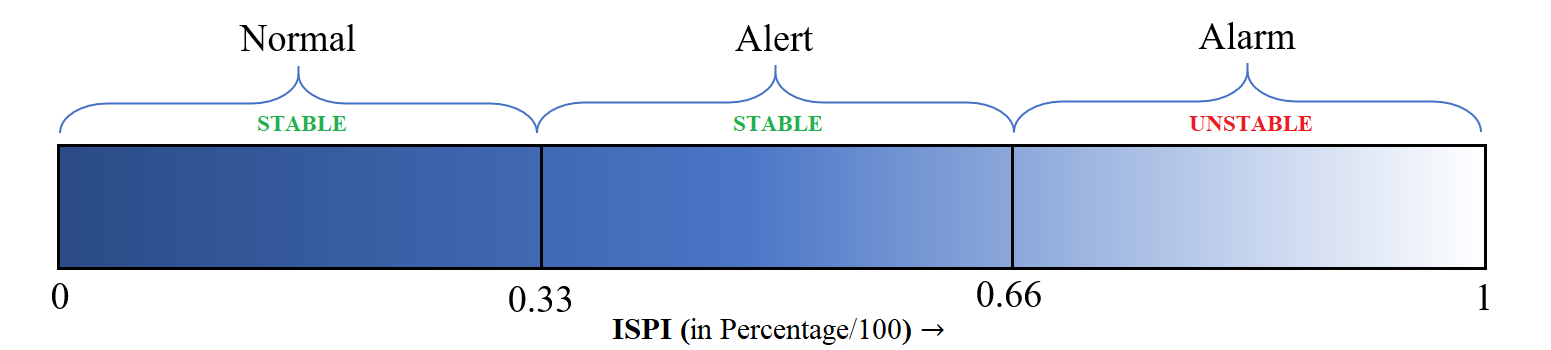
\includegraphics[width=12 cm]{ISPI Categories.png}
	\caption{Stability Prediction Index Categories}
	\label{ISPI Categories}
	\end{figure}

\section{Problem Formulation}
A power system is made up of a few basic components that are all interrelated. The generators, transmission lines, loads, transformer, static VAR compensators, and HVDC lines are the most important. There might be a couple of disturbances during the activity of the generators, for example, upheld movements in the speed or intermittent varieties in the force applied to the generator. These annoyances may cause a change in voltage or frequency, which may affect various components of the interconnected power system. Lightning and other external elements can also wreak havoc on the power system and transfer capacity between frameworks. Faults is the name given to this slew of disquieting influences. If the typical frequency of oscillation harmonises with the frequency oscillation of the generators, an fault causes the motor to lose synchronism. In light of these factors, synchronism is a necessary requirement for a power system with stability. Other crucial variables include steady-state stability, transient stability, music and unsettling impact, voltage breakdown, and a lack of reactive power, among others. The ability of an interconnected power system to return to its generally expected or stable activity after being subjected to some sort of adversity. Framework stability is defined as the ability of the framework to provide the heap and keep the many synchronous machines in sync under various conditions without the assistance of anybody else. The investigations are helpful in determining things like why a need has emerged. Voltage level, critical clearing time of circuit breakers. So, proposed methods of evaluating system is by considering Catastrophic Indicator computation and to take necessary steps looking at stability of the system in due time. Importance of the discussed formulas are they are easy and simple and easy to execute once the required parameters are obtained in case of proper Algorithm is there to execute all indicators. 